\documentclass[a4paper,11pt]{article}

\usepackage[utf8]{inputenc}
\usepackage[T1]{fontenc}
\usepackage[margin=2.5cm]{geometry}
\usepackage{amsmath}
\usepackage{xcolor}
\usepackage{hyperref}
\usepackage{graphicx}

% code block style
\usepackage{listings}
\usepackage{xcolor}

\definecolor{codegreen}{rgb}{0,0.6,0}
\definecolor{codegray}{rgb}{0.5,0.5,0.5}
\definecolor{codepurple}{rgb}{0.58,0,0.82}
\definecolor{backcolour}{rgb}{0.95,0.95,0.92}

\lstdefinestyle{mystyle}{
    backgroundcolor=\color{backcolour},
    commentstyle=\color{codegreen},
    keywordstyle=\color{magenta},
    numberstyle=\tiny\color{codegray},
    stringstyle=\color{codepurple},
    basicstyle=\ttfamily\footnotesize,
    breakatwhitespace=false,
    breaklines=true,
    captionpos=b,
    keepspaces=true,
    numbers=left,
    numbersep=5pt,
    showspaces=false,
    showstringspaces=false,
    showtabs=false,
    tabsize=2
}
\lstset{style=mystyle}

% Settings
\usepackage[sc]{titlesec}
\newcommand{\comment}[1]{\noindent \textcolor{blue}{\textit{#1}} \par}

% Header information
\title{\Large{\sc{Performance Engineering}}\\[2mm] Lab 6}
\author{Jort Oosterveld S5545781 \& Sergiu Preda S6778542 \\ Group 11}

\begin{document}
\setlength\parindent{0pt}

\maketitle

\section{Parallelized memory access}
\subsection{a)}

The reference STREAM benchmark (unmodified) was compiled using \texttt{gcc -O3 -fopenmp -mcpu=native} and run on one cluster node (2 Kunpeng~920 processors, 128 cores, 4 NUMA domains of 32 cores). THP is set to \texttt{always} on this node. Two array lengths were used: $N=1024$ (24\,KB for the three arrays, fits in L1D) and $N=10^8$ (2.4\,GB). The latter is larger than the required $2^{22}$, to be sure that nothing is served from the L3 cache. The threads were set with \texttt{OMP\_NUM\_THREADS} and not bound. Each point in figure \ref{fig:threads} is the median of 10 runs of the triad kernel, the bars show the minimum and maximum.

\begin{figure}[ht]
    \centering
    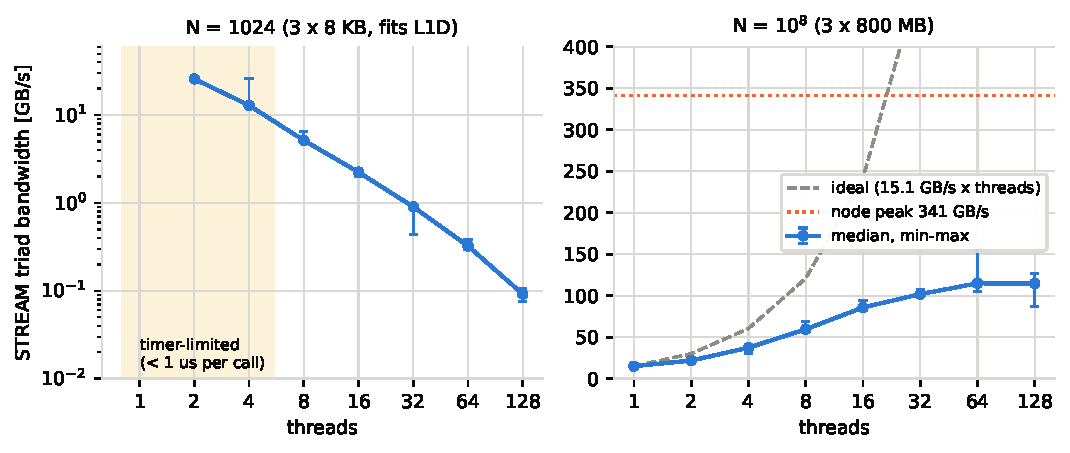
\includegraphics[width=\linewidth]{sources/fig_ex1_threads.pdf}
    \caption{STREAM triad bandwidth as a function of the number of threads. The values in the shaded area ($N=1024$, 1--4 threads) are limited by the 1\,$\mu$s resolution of the STREAM timer and are not meaningful.}
    \label{fig:threads}
\end{figure}

For $N=10^8$ one thread reaches 15\,GB/s, and the bandwidth grows less than linearly with the number of threads until it saturates at about 115\,GB/s from 64 threads on, which is a third of the theoretical 341\,GB/s of the node. A single core can only have a limited number of memory requests in flight, so multiple threads are needed to use the memory channels, but once they are saturated more threads do not help, they only increase the variation between runs.

For $N=1024$ the data stays in L1D, and the bandwidth \emph{decreases} with the number of threads: 5\,GB/s at 8 threads, 0.09\,GB/s at 128 threads. The work per thread is only a fraction of a microsecond, so what is measured is the cost of starting the parallel region and the barrier at the end of the loop. This grows with the number of threads, from 5\,$\mu$s per call at 8 threads to 267\,$\mu$s at 128 threads. Parallelizing such a short loop does not pay off.

\subsection{b)}

The same benchmark was used with \texttt{OMP\_PLACES=cores}, and \texttt{OMP\_PROC\_BIND} set to \texttt{false}, \texttt{true}, \texttt{master}, \texttt{close} and \texttt{spread}. With 128 threads every core gets one thread, so the settings can hardly differ there; therefore 32 and 64 threads were also used. The CPU of each thread was checked during a run (\texttt{ps -L -o psr}). The results are in figure \ref{fig:bind}.

\begin{figure}[ht]
    \centering
    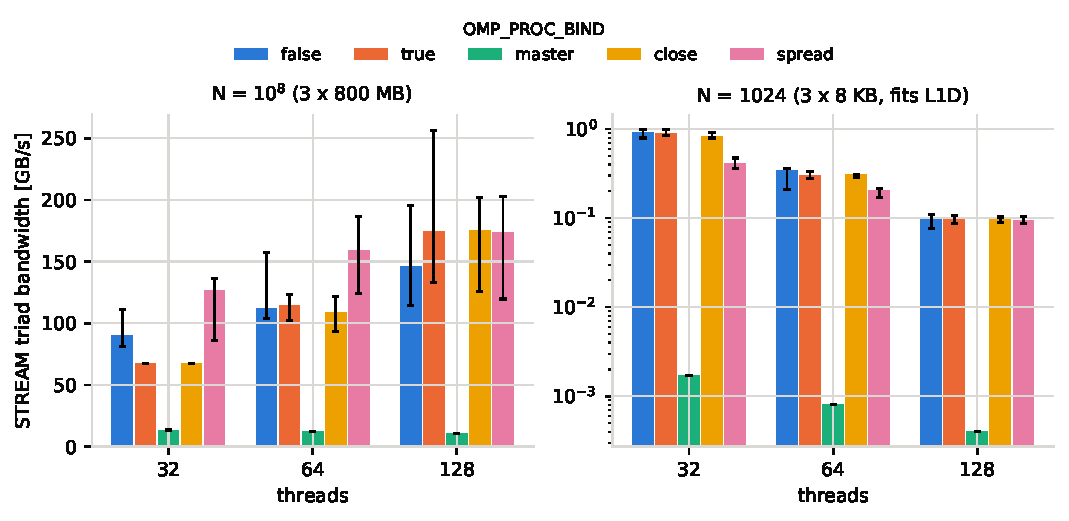
\includegraphics[width=\linewidth]{sources/fig_ex1_bind.pdf}
    \caption{STREAM triad bandwidth for the five settings of \texttt{OMP\_PROC\_BIND} (median of 10 runs, bars: min--max). Left: $N=10^8$. Right: $N=1024$ (log scale).}
    \label{fig:bind}
\end{figure}

For $N=10^8$ the bandwidth depends on how many NUMA domains, and with them memory controllers, are used. \texttt{close} fills the domains one by one, so 32 threads use only one domain and give 67\,GB/s. \texttt{spread} puts 8 threads in each of the 4 domains and gives 127\,GB/s, with the same number of threads. With 128 threads \texttt{close}, \texttt{true} and \texttt{spread} are the same placement and give the same result (about 175\,GB/s). For $N=1024$ the time is dominated by synchronization, and there \texttt{close} is faster than \texttt{spread} (0.84 against 0.41\,GB/s at 32 threads), because the threads are in the same NUMA domain.

\begin{itemize}
    \item \textbf{false}
        \begin{itemize}
            \item \textbf{pros:} No tuning needed, the OS can balance the load, and it spreads the threads over the domains (90\,GB/s at 32 threads).
            \item \textbf{Cons:} Threads can migrate and lose their cached data and the first-touch locality; the results vary the most (115--196\,GB/s at 128 threads).
        \end{itemize}
    \item \textbf{true}
        \begin{itemize}
            \item \textbf{pros:} Threads are pinned, so the result is reproducible.
            \item \textbf{Cons:} The policy is left to the implementation; with GCC it gave exactly the same placement as \texttt{close}.
        \end{itemize}
    \item \textbf{master}
        \begin{itemize}
            \item \textbf{pros:} All threads stay near the data of the master thread.
            \item \textbf{Cons:} All threads run on the core of the master: the bandwidth of one thread (11--14\,GB/s), and with $N=1024$ a barrier takes milliseconds. Worst of all settings.
        \end{itemize}
    \item \textbf{close}
        \begin{itemize}
            \item \textbf{pros:} Neighbouring threads share caches and synchronize cheaply.
            \item \textbf{Cons:} With fewer threads than cores only few memory controllers are used (67\,GB/s at 32 threads).
        \end{itemize}
    \item \textbf{spread}
        \begin{itemize}
            \item \textbf{pros:} Uses all memory controllers already with few threads, best for memory-bound loops (159\,GB/s at 64 threads, against 109 for \texttt{close}).
            \item \textbf{Cons:} Neighbouring threads share no caches, and synchronization across domains is more expensive. No advantage when all cores are used.
        \end{itemize}
\end{itemize}

Even with identical binding, the results for 128 threads vary between runs (\texttt{true}: 133, 175 and once 256\,GB/s). The threads are on the same cores every time, so the memory pages must end up in different places; THP \texttt{always} is a likely cause, but we did not test this.

\section{OpenMP parallelization and scheduling policies}

\subsection{a)}

The full source code of the paralellized mxv, including benchmark, can be found in listing \ref{lst:paralellization_source}. A clarification: this benchmark does not measure only the effect of paralellism, because the SIMD reduction was also added, in addition to the accumulator. Both of these things speed up the processing for the mxv. The baseline is just meant as a reference without any optimizations.

The code was compiled using \texttt{gcc -O3 -march=native -fopenmp} on the cluster, and the threads were configured with \texttt{OMP\_NUM\_THREADS=128 OMP\_PLACES=cores OMP\_PROC\_BIND=spread}. The code was ran with parameters \texttt{M=32768}, \texttt{N=32768} and \texttt{ITERS=100}.

\subsection{b)}
I would propose a static schedule, partly because of the parallel memory initialization being static as well, and likely dividing the pages across threads the same way the calculation loop will. Another reason is that the workload is very regular, meaning each thread will perform close to the same amount of work. There is not much to gain with dynamic scheduling, if the static scheduling already splits the work up evenly.

\begin{itemize}
    \item \textbf{Static}
        \begin{itemize}
            \item \textbf{pros:} Very low scheduling overhead, good load balance because all rows have similar cost, good cache/NUMA locality, predictable.
            \item \textbf{Cons:} If workload turns out to be irregular, is slower.
        \end{itemize}
    \item \textbf{Dynamic}
        \begin{itemize}
            \item \textbf{pros:} Can balance irregular workloads well, useful when threads finish earlier, they can take on extra work.
            \item \textbf{Cons:} Extra runtime scheduling overhead, worse locality.
        \end{itemize}
    \item \textbf{Guided}
        \begin{itemize}
            \item \textbf{pros:} Lower scheduling overhead than fully dynamic scheduling, can still compensate for workload imbalance.
            \item \textbf{Cons:} Still more overhead and less predictable locality than static.
        \end{itemize}
\end{itemize}

\subsection{c)}
From the results in figure \ref{fig:parallel_mxv_results}, we see that all schedules lie quite close to one another. Static is the most stable in terms of execution time, as expected, due to predictable workload scheduling. What is unexpected is that the mean of both dynamic and guided are lower than that of static. Guided is the fastest. A possible explanation is that the threads do not get the same memory bandwidth. In this case, some threads might finish earlier, and the whole calculation will benefit from dynamic scheduling. Guided scheduling only adds less overhead, and since the workload is predictable, will do a better job.

\begin{figure}[ht]
    \centering
    \includegraphics[width=0.9\linewidth]{sources/parallel_mxv_cluster.png}
    \caption{Matrix-vector multiplication runtime on the cluster, with the no-paralellization mxv, and paralellized mxvs with scheduling policies: static, dynamic and guided.}
    \label{fig:parallel_mxv_results}
\end{figure}

\newpage
\begin{lstlisting}[language=C, label=lst:paralellization_source, caption=Source code for the OpenMP paralellization benchmarks]
#include <omp.h>
#include <stdio.h>
#include <stdlib.h>
#include <time.h>

#define NS_DIV 1000000000LL

void mxv(double *restrict y,
         double *restrict a,
         double *restrict x,
         size_t m, size_t n)
{
    for (size_t i=0; i<m; i++) {
        y[i] = 0.0;
        for (size_t j=0; j<n; j++) {
            y[i] += a[i*n+j] * x[j];
        }
    }
}

/* Three separate functions for the parallel implementation, because of simplicity.
 * We did not want to complicate the code and the running script with compile-time
 * if-statements for each schedule directive, and have to recompile the binary each time.
 */
void mxv_par_static(double *restrict y,
         double *restrict a,
         double *restrict x,
         size_t m, size_t n)
{
    #pragma omp parallel for default(none) shared(y,a,x,m,n) schedule(static)
    for (size_t i=0; i<m; i++) {

        double sum = 0.0; // local variable to avoid unnecessary memory writes
        size_t col = i * n; // don't recompute column each time
        #pragma omp simd reduction(+:sum)
        for (size_t j=0; j<n; j++) {
            sum += a[col+j] * x[j];
        }
        y[i] = sum;
    }
}

void mxv_par_dynamic(double *restrict y,
         double *restrict a,
         double *restrict x,
         size_t m, size_t n)
{
    #pragma omp parallel for default(none) shared(y,a,x,m,n) schedule(dynamic)
    for (size_t i=0; i<m; i++) {

        double sum = 0.0; // local variable to avoid unnecessary memory writes
        size_t col = i * n; // don't recompute column each time
        #pragma omp simd reduction(+:sum)
        for (size_t j=0; j<n; j++) {
            sum += a[col+j] * x[j];
        }
        y[i] = sum;
    }
}

void mxv_par_guided(double *restrict y,
         double *restrict a,
         double *restrict x,
         size_t m, size_t n)
{
    #pragma omp parallel for default(none) shared(y,a,x,m,n) schedule(guided)
    for (size_t i=0; i<m; i++) {

        double sum = 0.0; // local variable to avoid unnecessary memory writes
        size_t col = i * n; // don't recompute column each time
        #pragma omp simd reduction(+:sum)
        for (size_t j=0; j<n; j++) {
            sum += a[col+j] * x[j];
        }
        y[i] = sum;
    }
}

int main(int argc, char *argv[]) {
    if (argc != 4) {
        printf("Usage: %s <MAT_COLS> <MAT_ROWS> <iterations (unsigned int)>\n", argv[0]);
        return 1;
    }

    /* Trust the user that they will not input a stupid number, since he is me. */
    size_t N = strtoull(argv[1], NULL, 10);
    size_t M = strtoull(argv[2], NULL, 10);
    size_t max_it = strtoull(argv[3], NULL, 10);

    /* open csv file for results */
    FILE *results_csv = fopen("results.csv", "w");

    if (!results_csv) {
        perror("Could not open results.csv");
        return 1;
    }

    fprintf(results_csv, "iteration,paralellization_type,time_ns,result\n");

    // Allocate memory
    double *A = (double *)malloc(M * N * sizeof(double));
    double *x = (double *)malloc(N * sizeof(double));
    double *y = (double *)malloc(M * sizeof(double));

    if (!A || !x || !y) {
        printf("Memory allocation failed.\n");

        free(A);
        free(x);
        free(y);
        fclose(results_csv);

        return 1;
    }

    /* Parallel first-touch initialization. Possible limitation that pages might migrate
    * because of large serial access right after parallel static schedule allocate.
    */
    #pragma omp parallel default(none) shared(A, x, y, M, N)
    {
        #pragma omp for schedule(static) // only static, not the other scheduling policies,
        // because we cannot predict which pages are processed by which threads later
        for (size_t i=0; i < M; i++) {
            size_t row = i * N;

            for (size_t j=0; j < N; j++) {
                A[row + j] = 1.0;
            }
        }

        #pragma omp for schedule(static)
        for (size_t i=0; i < N; i++) {
            x[i] = 2.0;
        }

        #pragma omp for schedule(static)
        for (size_t i=0; i < M; i++) {
            y[i] = 0.0;
        }
    }

    /* =========================== Baseline benchmark =========================== */

    for (size_t i=0; i<max_it; i++) {
        // start timer
        struct timespec start, end;
        clock_gettime(CLOCK_MONOTONIC, &start);
        // Run the blocked matrix-vector multiplication
        mxv(y, A, x, M, N);
        clock_gettime(CLOCK_MONOTONIC, &end);
        long long time_taken_ns = (end.tv_sec - start.tv_sec) * NS_DIV + (end.tv_nsec - start.tv_nsec);

        fprintf(results_csv, "%zu,baseline,%lld,%lf\n", i, time_taken_ns,y[0]);
        printf("Execution time: %lld ns\n", time_taken_ns);

        // Print a single value to prevent dead-code elimination
        printf("Result y[0]: %f\n", y[0]);
    }

    /*=========================== Paralellization using Static ===========================*/

    for (size_t i=0; i<max_it; i++) {
        // start timer
        struct timespec start, end;
        clock_gettime(CLOCK_MONOTONIC, &start);
        // Run the blocked matrix-vector multiplication
        mxv_par_static(y, A, x, M, N);
        clock_gettime(CLOCK_MONOTONIC, &end);
        long long time_taken_ns = (end.tv_sec - start.tv_sec) * NS_DIV + (end.tv_nsec - start.tv_nsec);

        fprintf(results_csv, "%zu,parallel_static,%lld,%lf\n", i, time_taken_ns,y[0]);
        printf("Execution time: %lld ns\n", time_taken_ns);

        // Print a single value to prevent dead-code elimination
        printf("Result y[0]: %f\n", y[0]);
    }

    /*=========================== Paralellization using Dynamic ===========================*/

    for (size_t i=0; i<max_it; i++) {
        // start timer
        struct timespec start, end;
        clock_gettime(CLOCK_MONOTONIC, &start);
        // Run the blocked matrix-vector multiplication
        mxv_par_dynamic(y, A, x, M, N);
        clock_gettime(CLOCK_MONOTONIC, &end);
        long long time_taken_ns = (end.tv_sec - start.tv_sec) * NS_DIV + (end.tv_nsec - start.tv_nsec);

        fprintf(results_csv, "%zu,parallel_dynamic,%lld,%lf\n", i, time_taken_ns,y[0]);
        printf("Execution time: %lld ns\n", time_taken_ns);

        // Print a single value to prevent dead-code elimination
        printf("Result y[0]: %f\n", y[0]);
    }

    /*=========================== Paralellization using Guided ===========================*/

    for (size_t i=0; i<max_it; i++) {
        // start timer
        struct timespec start, end;
        clock_gettime(CLOCK_MONOTONIC, &start);
        // Run the blocked matrix-vector multiplication
        mxv_par_guided(y, A, x, M, N);
        clock_gettime(CLOCK_MONOTONIC, &end);
        long long time_taken_ns = (end.tv_sec - start.tv_sec) * NS_DIV + (end.tv_nsec - start.tv_nsec);

        fprintf(results_csv, "%zu,parallel_guided,%lld,%lf\n", i, time_taken_ns,y[0]);
        printf("Execution time: %lld ns\n", time_taken_ns);

        // Print a single value to prevent dead-code elimination
        printf("Result y[0]: %f\n", y[0]);
    }

    // Cleanup
    fclose(results_csv);

    free(A);
    free(x);
    free(y);

    return 0;
}
\end{lstlisting}

\end{document}
